\subsection{Runtime Adaptation}
\label{sec:runtime}

At runtime, \sysname{} matches data rate to available bandwidth to minimize
latency and uses Pareto-optimal configurations to maximize accuracy.

\begin{figure}
  \centering
  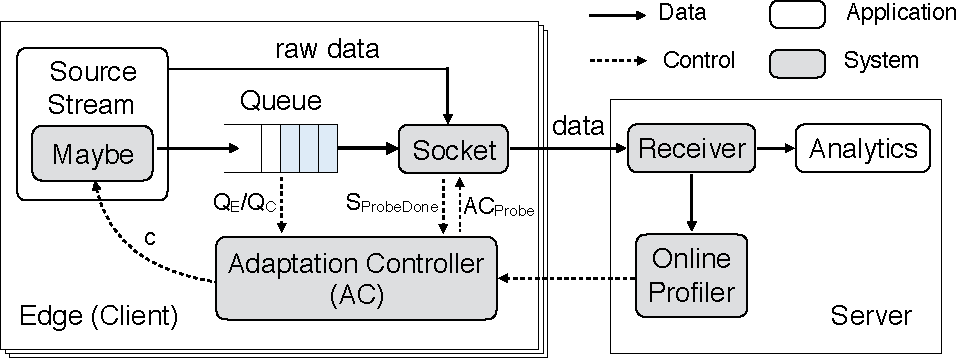
\includegraphics[width=\linewidth]{figures/runtime-adaptation.pdf}
  \caption{Runtime adaptation system architecture.}
  \label{fig:runtime}
\end{figure}

\autoref{fig:runtime} shows our runtime system architecture. \sysname{}
applications' source contains a \texttt{Maybe} module derived from all \maybe{}
operators. This module allows the controller to update the level of
degradation. Data generated by the source is then enqueued to \texttt{Queue} and
subsequently dequeued by \texttt{Socket}, which sends data over the network
using TCP. When the data generation rate exceeds \texttt{Socket}'s departure
rate, the queue grows. In this case, the adaptation controller (AC) queries the
estimated bandwidth from \texttt{Socket} and regulates the source stream by
updating the configuration. After the data is sent through the network,
\texttt{Receiver} delivers data to the application analytics. \texttt{Receiver}
also performs congestion detection and extracts raw data, if it presents.  It
tracks minimal latency (similar to how BBR tracks
\texttt{RTprop}~\cite{cardwell2017bbr} within a filter window) and reports
sudden latency spikes to clients as congestion signalling. Raw data is only
transmitted when the queue is empty and online profiling is enabled. After a new
profile is learned by the online profiler, it is fed back to AC for subsequent
adaptation.

\begin{figure}
  \begin{subfigure}[t]{\columnwidth}
    \centering
    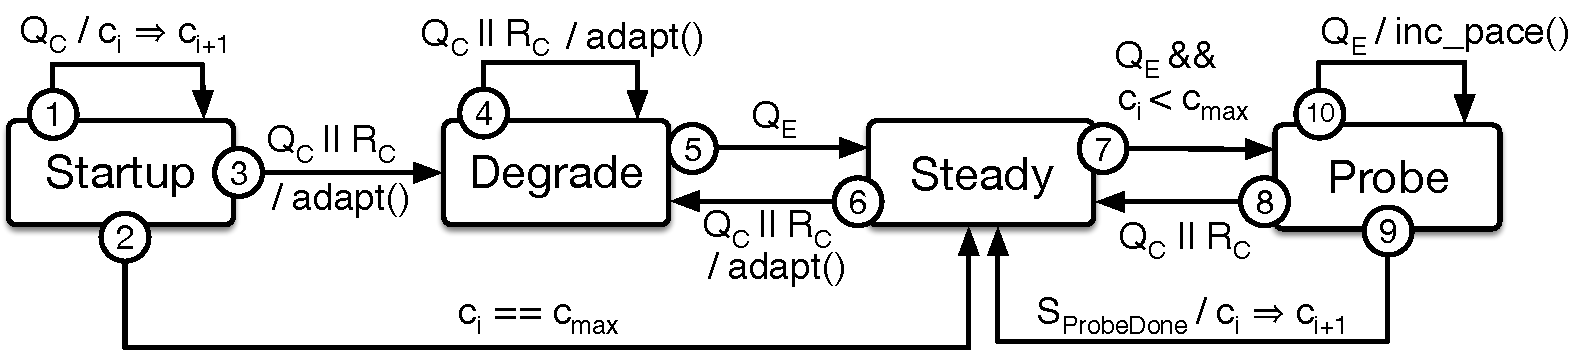
\includegraphics[width=\columnwidth]{figures/cc.pdf}
    \caption{Rate adaptation as a state machine.}
    \vspace{1em}
    \label{fig:cc-sm}
  \end{subfigure}
  \\
  \centering
  \begin{subfigure}[t]{\columnwidth}
    \centering
    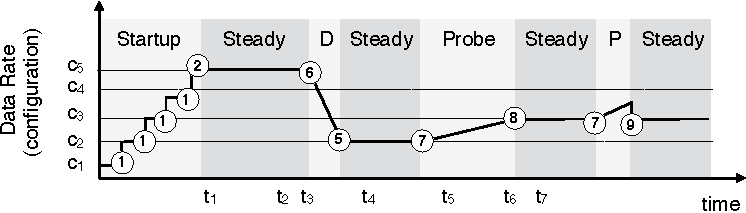
\includegraphics[width=0.9\columnwidth]{figures/cc2.pdf}
    \caption{An example illustrating the adaptation algorithm.}
    \label{fig:cc-ex}
  \end{subfigure}
  \caption{Runtime adaptation algorithm.}
  \label{fig:cc}
\end{figure}

\autoref{fig:cc-sm} shows the adaptation algorithm with a state machine model
and \autoref{fig:cc-ex} shows the state transitions with an example. AC loads
the profile and sorts all configurations with an ascending order of bandwidth
demand, resulting in a list $[c_1, \dots, c_{\max}]$.  These configurations
follow a total order: $c_i < c_j$ if $B(c_i) < B(c_j)$.  We denote the current
configuration as $c_i$ and the next $c_{i+1}$.  AC receives messages from the
\texttt{Queue}: message \qe{} when the queue is empty and $\text{Q}_\text{C}$
when queued items exceed a threshold. AC can query \texttt{Socket} for delivery
rate $R$ (arrow not shown) or request the source to probe
($\text{AC}_{\text{Probe}}$) for a target bandwidth, often $B(c_{i+1})$. If
there is no queue built up during the probing and $R > B(c_{i+1})$,
\texttt{Socket} sends back \spd{}. The reactions in each state are as follows:

\begin{itemize}[leftmargin=*, topsep=3pt, itemsep=0pt]

\item \textbf{Startup: rapid growth.} \sysname{} starts with $c_1$ and grows the
  rate ($c_i \Rightarrow c_{i+1}$) upon each \qe{}. The growth stops at
  $c_{\max}$ (to \texttt{Steady}) or if it receives \qc{}/\rc{} (to
  \texttt{Degrade}).

\item \textbf{Degrade: reacting to congestion.} Congestion is detected in two
  ways: (1) when \texttt{Queue} grows and exceeds a threshold, AC receives
  \qc{}; (2) when \texttt{Receiver} detects latency spikes, AC receives
  \rc{}. During congestion, AC runs the \texttt{adapt()} procedure by updating
  \texttt{Maybe} with the maximum-allowed $c$ that satisfies $B(c) < \alpha R$,
  where $\alpha \in (0, 1)$ and $R$ is \texttt{Socket}'s current delivery
  rate. A smaller $\alpha$ allows a quicker draining of the queue. After the
  congestion is resolved (\qe{} received), \sysname{} changes to
  \texttt{Steady}.

\item \textbf{Steady: low latency delivery.} \sysname{} achieves low latency by
  spending most of the time in the \texttt{Steady} state. It changes to
  \texttt{Degrade} when congestion occurs. If $c < c_{\max}$ and it receives
  \qe{}, AC enters the \texttt{Probe} state to check for more available
  bandwidth.

\item \textbf{Probe: more bandwidth for a higher accuracy.} Advancing the
  configuration directly causes a drastic latency increase when
  $B(c_{i+1}) \gg B(c_i)$. To allow a smooth increase, AC requests
  \texttt{Socket} to probe by sending additional traffic controlled by
  \texttt{probe\_gain} (in \texttt{inc\_pace()}, similar to
  BBR~\cite{cardwell2017bbr}). \sysname{} stops probing under two conditions:
  (1) upon \spd{}, it advances $c_i$; (2) upon \qc{} or \rc{}, it returns to
  \texttt{Steady}.

\end{itemize}

\para{Comparison with JetStream (only runtime).} $(1)$ \sysname{} and JetStream
use different feedback signals for rate adaptation. \sysname{} uses a direct
measurement of delivery rate to select an appropriate configuration that
satisfies the bandwidth constraint. In contrast, JetStream employs a
latency-based measure of capacity ratio, which only indirectly reflects
available bandwidth and is less accurate. $(2)$ \sysname{} has an explicit probe
phase while JetStream changes its policy immediately after capacity ratio
changes: it easily winds up overcompensating and the system will
oscillate. \fixme{Tone down, e.g., it may over-react and the system is susceptible
to oscillate.}
$(3)$ \sysname{} supports online profiling to keep the profile
updated while policies in JetStream are fixed after development time. In
\autoref{sec:runtime-adaptation}, we present the evaluation between two runtime
systems when using the \textit{same} Pareto-optimal policies generated by \sysname{}'s
profiler: the comparison between
\sysname{} and JetStream++.

\subsection{Resource Allocation \& Fairness}

In addition to rate adaptation, the profile is also useful for controlling a
single application's bandwidth usage or allocating resources among competing
tasks.

For individual applications, developers can pin-point a configuration for a
given bandwidth or accuracy goal. They can also specify a criterion to limit
effective configurations. For example, \sysname{} can enforce an upper bound on
the bandwidth consumption. In this way, applications can control their bandwidth
costs while using the profile to maximize accuracy.

For multiple applications, their profiles allow novel bandwidth allocation
schemes such as utility fairness. Different from traditional resource fairness
with which applications get equal share of bandwidth, utility fairness aims to
maximize the \textit{minimal} application accuracy. With the profiles, bandwidth
allocation is equivalent to finding proper configuration $c^t$ for application
$t$. We formulate utility fairness as follows:

%% Pick one based on the space

\begin{equation}
 \label{eq:multitask}
 \underset{c^t}{\max} \; \min({A^t(c^t)})
 \;
 \text{s.t.}
 \;
 \sum_t{B^t(c^t)} < R
\end{equation}

% \begin{equation}
%  \label{eq:multitask}
%  \begin{aligned}
%     & \underset{c^t}{\text{maximize}} & & \min({A^t(c^t)}) & & \\
%     & \text{subject to} & & \sum_t{B^t(c^t)} < R & & \\
%  \end{aligned}
% \end{equation}

Solving this optimization is computationally hard. \sysname{} uses a heuristics
approach. It starts with $c^t_1$ and improves the application $t$ with the worst
accuracy. This process repeats until all available bandwidth is allocated. \fixme{cite
the method}

%%% Local Variables:
%%% mode: latex
%%% TeX-master: "awstream"
%%% End:
